\documentclass[aspectratio=169,11pt]{beamer}
\def\courseweek{10}
% Shared style for the Introduction to Information Geometry lecture slides.
% Compile the lecture .tex files from this directory.
\providecommand{\courseweek}{1}
\usepackage[T1]{fontenc}
\usepackage[utf8]{inputenc}
\usepackage[sc]{mathpazo}
\renewcommand{\sfdefault}{lmss}
\renewcommand{\ttdefault}{lmtt}
\usepackage{amsmath,amssymb,mathtools}
\usepackage{tikz}
\usetikzlibrary{arrows.meta,calc,positioning}
\usepackage{pgfplots}
\pgfplotsset{compat=1.18}
\usepackage{booktabs}

\definecolor{courseink}{HTML}{173749}
\definecolor{coursemuted}{HTML}{526674}
\definecolor{courseteal}{HTML}{0E7287}
\definecolor{coursecopper}{HTML}{B66B43}
\definecolor{courseline}{HTML}{D4E0E3}
\definecolor{coursepale}{HTML}{EFF5F5}

\setbeamercolor{normal text}{fg=courseink,bg=white}
\setbeamercolor{structure}{fg=courseteal}
\setbeamercolor{frametitle}{fg=courseink,bg=white}
\setbeamercolor{title}{fg=courseink}
\setbeamercolor{subtitle}{fg=coursemuted}
\setbeamercolor{block title}{fg=courseink,bg=white}
\setbeamercolor{block body}{fg=courseink,bg=white}
\setbeamercolor{alerted text}{fg=coursecopper}
\setbeamerfont{title}{family=\rmfamily,series=\bfseries,size=\fontsize{32}{37}}
\setbeamerfont{frametitle}{family=\rmfamily,series=\bfseries,size=\fontsize{26}{31}}
\setbeamerfont{normal text}{size=\fontsize{18}{22}}
\setbeamerfont{subtitle}{size=\fontsize{17}{21}}
\setbeamersize{text margin left=0.78cm,text margin right=0.78cm}
\setbeamertemplate{navigation symbols}{}
\setbeamertemplate{itemize items}[circle]
\setbeamertemplate{enumerate items}[default]
\setbeamertemplate{blocks}[default]
\setlength{\parskip}{0.22em}
\setbeamertemplate{footline}{%
  \leavevmode\hbox to \paperwidth{\hspace{.78cm}%
  {\color{coursemuted}\fontsize{8.5}{10}\selectfont Introduction to Information Geometry \hspace{.32cm} / \hspace{.32cm} Week \courseweek}%
  \hfill{\color{coursemuted}\fontsize{8.5}{10}\selectfont \insertframenumber\hspace{.17cm}/\hspace{.17cm}\inserttotalframenumber}\hspace{.78cm}}%
  \vskip.17cm
}
\setbeamertemplate{frametitle}{%
  \vspace{.13cm}
  \insertframetitle\par
  \vspace{.08cm}
}
\setbeamertemplate{title page}{%
  \vspace*{1.00cm}
  {\color{courseteal}\fontsize{10}{13}\selectfont\bfseries
  INTRODUCTION TO INFORMATION GEOMETRY\par}
  \vspace{.40cm}
  {\usebeamerfont{title}\usebeamercolor[fg]{title}\inserttitle\par}
  \vspace{.22cm}
  {\usebeamerfont{subtitle}\usebeamercolor[fg]{subtitle}\insertsubtitle\par}
  \vfill
  {\color{coursemuted}\fontsize{13}{16}\selectfont Christopher Lee\par}
  \vspace{.34cm}
}

\pgfplotsset{
  courseplot/.style={
    width=11.05cm,
    height=5.15cm,
    axis line style={coursemuted!75},
    tick style={coursemuted!65},
    ticklabel style={font=\scriptsize,color=coursemuted},
    label style={font=\normalsize,color=courseink},
    grid=major,
    major grid style={courseline!70,line width=.4pt},
    line width=1.45pt,
    legend style={font=\small,draw=none,fill=none,at={(.98,.03)},anchor=south east},
    clip=true
  }
}

\newcommand{\highlightmath}[1]{{\color{courseteal}#1}}
\newcommand{\thinrule}{\par\vspace{.25cm}{\color{courseline}\rule{\linewidth}{.8pt}}\par}

% A one-dimensional state space.  x=0 and x=1 are placed at 0 and 9 units.
\newcommand{\stateinterval}[1]{%
 \begin{tikzpicture}[x=1cm,y=1cm]
   \draw[courseink,line width=1.25pt] (0,0)--(9,0);
   \foreach \pos/\lab in {0/0,9/1} {
     \fill[courseink] (\pos,0) circle(2.7pt);
     \node[below=9pt,text=coursemuted] at (\pos,0) {\(\lab\)};
   }
   #1
 \end{tikzpicture}%
}

% Paired pages are separate frames in the PDF, with matching titles.
% Supply the whole frame body for each version; the instructor may edit them
% independently without changing overlay logic.
\newcommand{\coursepair}[3]{%
  \begin{frame}{#1}#2\end{frame}%
  \begin{frame}{#1}#3\end{frame}%
}

% Equilateral representation of the categorical simplex, in barycentric
% coordinates with vertices A=(0,0), B=(1,0), C=(1/2,sqrt(3)/2).
\newcommand{\coursesimplex}[1]{%
 \begin{tikzpicture}[scale=4.9]
  \fill[coursepale] (0,0)--(1,0)--(.5,.8660254)--cycle;
  \draw[courseink,line width=.65pt] (0,0)--(1,0)--(.5,.8660254)--cycle;
  \node[below left,font=\small] at (0,0) {A};
  \node[below right,font=\small] at (1,0) {B};
  \node[above,font=\small] at (.5,.8660254) {C};
  #1
 \end{tikzpicture}%
}

\title{Gaussian Scores and the Hyperbolic Metric}
\subtitle{Week 10 \(\cdot\) Lecture 1}
\date{}
\begin{document}
\begin{frame}[plain]\titlepage\end{frame}

\begin{frame}{From probability vectors to density curves}
A continuous random variable has a density \(\rho(x)\) satisfying
\[
\rho(x)\geq0,\qquad \int_{-\infty}^{\infty}\rho(x)\,dx=1.
\]
\vspace{.45cm}
For an interval \([a,b]\), the probability is its density area:
\[
\Pr(a\leq X\leq b)=\int_a^b\rho(x)\,dx.
\]
\end{frame}

\begin{frame}{The two-parameter Gaussian family}
The normal density is
\[
\highlightmath{\rho(x;\mu,\sigma)=\frac1{\sigma\sqrt{2\pi}}
\exp\!\left[-\frac{(x-\mu)^2}{2\sigma^2}\right]},
\quad\sigma>0.
\]
\vspace{.44cm}
The parameter \(\mu\) locates the center;
\(\sigma\) controls the standard deviation.
\vspace{.40cm}
Each point \((\mu,\sigma)\) specifies an entire probability law.
\end{frame}

\begin{frame}{Moving a point changes a density}
\vspace{-.22cm}
\begin{center}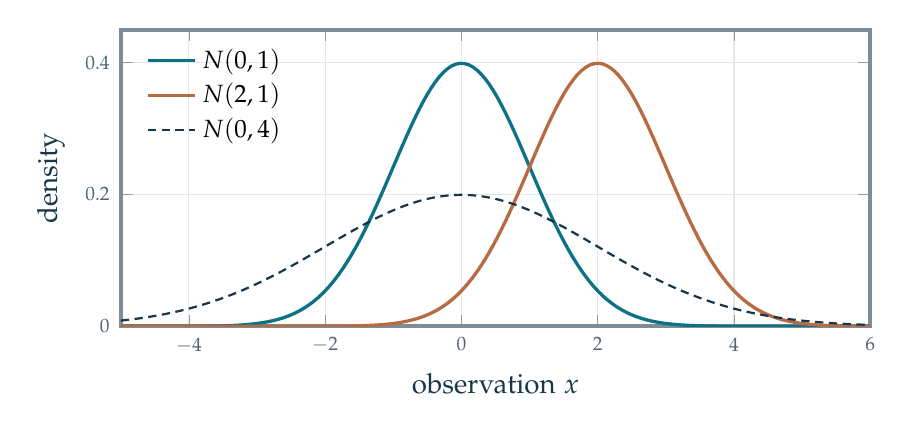
\begin{tikzpicture}
\begin{axis}[courseplot,width=11.1cm,height=5.35cm,xmin=-5,xmax=6,
 ymin=0,ymax=.45,xlabel={observation \(x\)},ylabel={density},
 legend style={font=\small,draw=none,at={(.02,.98)},anchor=north west}]
\addplot[courseteal,very thick,domain=-5:6,samples=180]{exp(-x^2/2)/sqrt(2*pi)};
\addlegendentry{\(N(0,1)\)}
\addplot[coursecopper,very thick,domain=-5:6,samples=180]{exp(-(x-2)^2/2)/sqrt(2*pi)};
\addlegendentry{\(N(2,1)\)}
\addplot[courseink,densely dashed,thick,domain=-5:6,samples=180]{exp(-x^2/8)/(2*sqrt(2*pi))};
\addlegendentry{\(N(0,4)\)}
\end{axis}\end{tikzpicture}\end{center}
\end{frame}

\begin{frame}{Expectation becomes an integral}
For a density \(\rho(x)\), the expected value of a function is
\[
\highlightmath{E[g(X)]=\int_{-\infty}^{\infty}g(x)\rho(x)\,dx}.
\]
\vspace{.48cm}
For a Gaussian, introduce the standardized variable
\[
Z=\frac{X-\mu}{\sigma}.
\]
\vspace{.36cm}
It has mean zero and variance one.
\end{frame}

\begin{frame}{The moments we need}
Odd standardized moments vanish by symmetry:
\[
E[Z]=E[Z^3]=0.
\]
\vspace{.48cm}
Integration by parts gives
\[
\highlightmath{E[Z^2]=1,\qquad E[Z^4]=3}.
\]
\vspace{.45cm}
These four expectations are enough to compute
the Gaussian Fisher information matrix.
\end{frame}

\begin{frame}{The Gaussian log density}
Taking the logarithm turns the product and exponential
in the Gaussian density into a sum:
\[
\ell(x;\mu,\sigma)
=-\ln\sigma-\frac12\ln(2\pi)
-\frac{(x-\mu)^2}{2\sigma^2}.
\]
\vspace{.55cm}
The score in each parameter direction is the derivative
of this log density.
\end{frame}

\coursepair{Calculate the two score functions}{
Starting with
\[
\ell=-\ln\sigma-\tfrac12\ln(2\pi)
-\frac{(x-\mu)^2}{2\sigma^2},
\]
\vspace{.31cm}
find \(S_\mu=\partial_\mu\ell\) and
\(S_\sigma=\partial_\sigma\ell\).
}{
Starting with the Gaussian log density,
\[
\highlightmath{S_\mu=\frac{x-\mu}{\sigma^2}},
\qquad
\highlightmath{S_\sigma=-\frac1\sigma
+\frac{(x-\mu)^2}{\sigma^3}}.
\]
\vspace{.44cm}
Equivalently, \(S_\mu=Z/\sigma\) and
\(S_\sigma=(Z^2-1)/\sigma\).
}

\begin{frame}{The scores have mean zero}
In standardized form, the two scores are
\[
S_\mu=\frac Z\sigma,\qquad
S_\sigma=\frac{Z^2-1}{\sigma}.
\]
\vspace{.4cm}
Therefore
\[
E[S_\mu]=\frac{E[Z]}\sigma=0,
\qquad E[S_\sigma]=\frac{E[Z^2]-1}\sigma=0.
\]
\end{frame}

\coursepair{Compute the Fisher matrix}{
The Fisher matrix is \(G_{ij}=E[S_iS_j]\).
\vspace{.38cm}
Use
\[
S_\mu=Z/\sigma,\qquad S_\sigma=(Z^2-1)/\sigma
\]
and \(E[Z^2]=1\), \(E[Z^3]=0\), \(E[Z^4]=3\).
\vspace{.27cm}
Find the three distinct matrix entries.
}{
The Fisher matrix is \(G_{ij}=E[S_iS_j]\), so
\[
G_{\mu\mu}=\frac1{\sigma^2},\qquad
G_{\mu\sigma}=0,\qquad
G_{\sigma\sigma}=\frac{3-2+1}{\sigma^2}.
\]
\vspace{.29cm}
Thus
\[
\highlightmath{G(\mu,\sigma)=\frac1{\sigma^2}
\begin{pmatrix}1&0\\0&2\end{pmatrix}}.
\]
}

\begin{frame}{The Gaussian Fisher line element}
For a small parameter change \((d\mu,d\sigma)\),
\[
\highlightmath{ds_F^2=\frac{d\mu^2+2\,d\sigma^2}{\sigma^2}}.
\]
\vspace{.47cm}
Mean and scale directions are orthogonal in this metric.
\vspace{.46cm}
The factor \(1/\sigma^2\) makes a fixed numerical change
statistically longer when the distribution is narrow.
\end{frame}

\coursepair{Compare two small Gaussian changes}{
At \(N(0,4)\), the standard deviation is \(\sigma=2\).
\vspace{.4cm}
Compare the Fisher lengths of
\[
(d\mu,d\sigma)=(h,0)
\quad\text{and}\quad(0,h).
\]
\vspace{.26cm}
Which change has greater length for the same \(|h|\)?
}{
At \(\sigma=2\), the squared lengths are
\[
\frac{h^2}{4}\quad\text{and}\quad\frac{2h^2}{4}.
\]
\vspace{.32cm}
Thus their lengths are
\[
\highlightmath{\frac{|h|}{2}}\quad\text{and}\quad
\highlightmath{\frac{|h|}{\sqrt2}}.
\]
\vspace{.16cm}
A scale change is \(\sqrt2\) times as long.
}

\begin{frame}{Rescale the horizontal coordinate}
Set
\[
u=\frac\mu{\sqrt2},\qquad v=\sigma>0.
\]
\vspace{.47cm}
The line element becomes
\[
\highlightmath{ds_F^2=2\frac{du^2+dv^2}{v^2}}.
\]
\vspace{.41cm}
The coordinate region is the upper half-plane \(v>0\).
\end{frame}

\begin{frame}{A hyperbolic geometry emerges}
The Poincar\'e half-plane metric is
\[
ds_{\mathbb H}^2=\frac{du^2+dv^2}{v^2}.
\]
\vspace{.42cm}
The Gaussian Fisher metric is twice this metric.
\vspace{.49cm}
Lengths scale by \(\sqrt2\); its constant Gaussian
curvature is \(\highlightmath{K=-1/2}\).
\end{frame}

\begin{frame}{Why traveling higher can be shorter}
The length of a parameter path \((u(t),v(t))\) is
\[
\highlightmath{L_F=\sqrt2\int\frac{\sqrt{u'(t)^2+v'(t)^2}}{v(t)}\,dt}.
\]
\vspace{.39cm}
At larger \(v\), the same Euclidean displacement
contributes less Fisher length.
\vspace{.39cm}
Geodesics use that variation in cost to connect distributions.
\end{frame}

\begin{frame}{Two spaces, two curvatures}
The interior of a finite categorical family is mapped
to part of a sphere of radius 2.
Its Fisher curvature is \(K=+1/4\).
\vspace{.49cm}
The full Gaussian family becomes a hyperbolic half-plane
with \(K=-1/2\).
\vspace{.49cm}
Both metrics come from the same construction:
expected products of score functions.
\end{frame}
\end{document}
